\documentclass[format=acmsmall, review=false]{acmart}

\usepackage{acm-ec-17}

\usepackage{booktabs} % For formal tables
\usepackage[ruled]{algorithm2e} % For algorithms
\usepackage{graphicx}     			% can better scale and rotate graphics than graphic package
\usepackage{multirow}               		% allows to have table cells on more than one row with "\multirow"
%\usepackage{amsmath, amsthm}	% !!! not for ACM template !!!
\usepackage{amssymb}                	% allows special symbols like "\nexists"
\usepackage{latexsym}               		% ? Dan
\usepackage{alltt}                  		% ? Dan
\usepackage{amsgen}                 	% ? Dan
\usepackage{amstext}               		% ? Dan
\usepackage{amscd}                  		% ? Dan
\usepackage{algorithmic}
\usepackage{url}
\usepackage{enumerate}
%\usepackage{cases}                  		% ? Dan
\usepackage{amsthm}
%\usepackage{mathtools}
%\usepackage{savesym}
\usepackage{amsmath}
\usepackage{tikz}
\usepackage{float}
\usepackage{enumitem}
\usepackage{mdwlist}
\usepackage{xspace}
\usetikzlibrary{arrows.meta}
%\savesymbol{iint}
%\usepackage{txfonts}
%\restoresymbol{TXF}{iint}
\usepackage{bm}                     	% bold Greek letters
\usepackage{upgreek}              
\usepackage{xspace}    
\usepackage{color}              
\usepackage{colortbl}    
\usepackage{tabularx}
\usepackage{aliascnt}  	
\usepackage{mdframed}
\usepackage{caption}
\usepackage{makecell}
\usepackage{tcolorbox}
\usepackage{float}                 % Should be included for hyperref according to Google Groups + algorithm + hyperref + float; in fact messes links to algorithms up
\graphicspath{ {experiments/} }
\usepackage{subcaption}

\renewcommand{\algorithmcfname}{ALGORITHM}
\SetAlFnt{\small}
\SetAlCapFnt{\small}
\SetAlCapNameFnt{\small}
\SetAlCapHSkip{0pt}
\IncMargin{-\parindent}

\begin{document}
% Title portion. Note the short title for running heads 
\title[Revenue Maximizing Algorithms for Query Pricing]{Revenue Maximization for Query Pricing : Approximation Algorithms and Practical Advances}  
\author{William Vickrey}
\affiliation{%
  \institution{College of William and Mary}}
\author{Edward Clarke}
\affiliation{%
  \institution{University of Virginia}
}
\author{Theodore Groves}
\affiliation{%
  \institution{Eaton Innovation Center}
}


\newcommand{\shaleen}[1]{{\color{blue} Shaleen: [{#1}]}}
\newcommand{\paris}[1]{{\color{red} Paris: [{#1}]}}
\newcommand{\todo}[1]{{\color{red} ToDo: {#1}}}
\newcommand{\cull}[1]{{\color{red} [{#1}]}}
\newcommand{\introparagraph}[1]{\textbf{#1.}}   
\newcommand{\cut}[1]{}

\newenvironment{packed_item}{
\begin{itemize}
   \setlength{\itemsep}{1pt}
   \setlength{\parskip}{0pt}
   \setlength{\parsep}{0pt}
}
{\end{itemize}}

\newenvironment{packed_enum}{
\begin{enumerate}
   \setlength{\itemsep}{1pt}
  \setlength{\parskip}{0pt}
   \setlength{\parsep}{0pt}
}
{\end{enumerate}}

\newenvironment{packed_grep}{
\begin{description}
   \setlength{\itemsep}{1pt}
   \setlength{\parskip}{0pt}
   \setlength{\parsep}{0pt}
}
{\end{description}}
              
\newcommand{\ie}{{\em i.e.}\xspace}
\newcommand{\eg}{{\em e.g.}\xspace}
\newcommand{\ea}{{\em et al.}\xspace}
\newcommand{\aka}{{\em a.k.a.}\xspace}

\newcommand{\dtr}[0]{\twoheadrightarrow}     
 
\newcommand{\bQ}[0]{\mathbf{Q}}       
\newcommand{\bD}[0]{\mathbf{D}}       
\newcommand{\bR}[0]{\mathbf{R}}       
\newcommand{\bU}[0]{\mathbf{U}}     
\newcommand{\bT}[0]{\mathbf{T}}     
\newcommand{\bA}[0]{\mathbf{A}}     
\newcommand{\bB}[0]{\mathbf{B}}     
\newcommand{\bAp}[0]{\mathbf{A}}     
\newcommand{\bBp}[0]{\mathbf{B}}     
\newcommand{\bC}[0]{\mathbf{C}}     
\newcommand{\bV}[0]{\mathbf{V}}   
\newcommand{\bG}[0]{\mathbf{G}}     
 
\newcommand{\mS}[0]{\mathcal{S}} 
\newcommand{\mI}[0]{\mathcal{I}}   
\newcommand{\mF}[0]{\mathcal{F}}   
\newcommand{\mH}[0]{\mathcal{H}}   
\newcommand{\mE}[0]{\mathcal{E}}   
\newcommand{\mV}[0]{\mathcal{V}}   
\newcommand{\mC}[0]{\mathcal{C}}      
\newcommand{\mM}[0]{\mathcal{M}}   
\newcommand{\mL}[0]{\mathcal{L}}   
\newcommand{\mP}[0]{\mathcal{P}}   

\newcommand{\APS}[0]{\textsf{APS}}   
\newcommand{\DPS}[0]{\textsf{DPS}} 
\newcommand{\QPS}[0]{\textsf{QPS}} 

\newcommand{\agr}[2]{\mS_{#1}(#2)} 
\newcommand{\dagr}[2]{{\mC}_{#1}(#2)} 
\newcommand{\setof}[2]{\{{#1}\mid{#2}\}}
\newcommand{\set}[1]{\{#1\}}   
\newcommand{\qb}[1]{\langle {#1} \rangle}   

\newcommand{\cmark}{\ding{51}}%
\newcommand{\xmark}{\ding{55}}%
\newcommand{\db}{\mathcal{D}}%
\newcommand{\upd}{\textsf{up}^\uparrow}

\newcommand{\ubp}{\textsf{UBP}}
\newcommand{\uip}{\textsf{UIP}}
\newcommand{\lpip}{\textsf{LPIP}}
\newcommand{\cip}{\textsf{CIP}}

\newcommand{\ra}[1]{\renewcommand{\arraystretch}{#1}}

\definecolor{Gray}{gray}{0.9}
\definecolor{cardinal}{rgb}{0.77, 0.12, 0.23}
\definecolor{bondiblue}{rgb}{0.0, 0.58, 0.71}
\definecolor{babyblue}{rgb}{0.54, 0.81, 0.94}
\definecolor{lightgreen}{rgb}{0.67, 0.94, 0.82}
\definecolor{maize}{rgb}{0.98, 0.93, 0.37}

\hypersetup{colorlinks,citecolor={cardinal}}  

%\DeclareRobustCommand{\hlrone}[1]{{\sethlcolor{babyblue}\hl{#1}}}
%\DeclareRobustCommand{\hlrtwo}[1]{{\sethlcolor{maize}\hl{#1}}}
%\DeclareRobustCommand{\hlrthree}[1]{{\sethlcolor{lightgreen}\hl{#1}}}

\newcommand{\hlrone}[1]{{\color{black} {#1}}}
\newcommand{\hlrtwo}[1]{{\color{black} {#1}}}
\newcommand{\hlrthree}[1]{{\color{black} {#1}}}
\newcommand{\cmr}[1]{{\color{black} {#1}}}


\begin{abstract}
In this paper, we present approximation algorithms for {\em query pricing} problem so as to maximize seller's revenue in the unlimited supply setting. We formulate the problem as an instance item pricing over {\em item hypergraph} where the buyers are {\em single minded} with subadditive valuations and investigate a variety of pricing strategies including {\em uniform item pricing} and {\em uniform bundle pricing}. \cite{guruswami2005profit} gave an $O(\log m + \log n)$ where $m$ is the number of customers and $n$ is the number of items with sum of all valuations as the upper bound. In our setting, we show that both item pricing and uniform bundle pricing exhibit a gap of $\Omega(m)$ from the optimal subadditive bundle pricing. Additionally, we investigate the revenue obtained using XOS pricing functions and show $O(\dots)$ approximation with a matching lower bound. We complement our theoretical results with extensive experiments on industry scale workloads. To this end, our experiments show that pricing algorithms behave very well in practice when valuations are drawn randomly from a variety of distributions including zipfian, normal and uniform distribution.
\end{abstract}

\maketitle
\section{Introduction}
\label{sec:intro}

The last decade or so has seen an explosion of data being collected from a variety of sources and across a broad range of areas. Many companies, including Bloomberg~\cite{bloomberg}, Twitter~\cite{twitterapi}, Lattice Data~\cite{lattice}, DataFinder~\cite{datafinder}, and Banjo~\cite{banjo} collect such data, which then sell as structured (relational) datasets. 
These datasets are also often sold through online {\em data markets}, which are web platforms for buying and selling data: examples include BDEX~\cite{bdex}, Salesforce~\cite{salesforce} and QLik DataMarket~\cite{qlik}. Even though data sellers and data markets offer an abundance of data products, the pricing schemes currently used are very simplistic. In most cases, a data buyer has only one option, to buy the whole dataset (or a bundle of datasets) at a fixed price. Alternatively, the dataset is split into multiple disjoint chunks, and each chunk is sold at a separate price. 

However, data buyers are commonly interested in extracting specific information from a dataset, and not in acquiring the whole dataset. Accessing this information can be often concisely captured through a {\em query}, or a sequence of queries. Selling the whole dataset to a fixed price forces the buyer to either pay for the query more than it is valued, or to choose to not access it. This means that valuable data is often not accessible to lay users, scientists, or entities with limited budgets, and moreover that data-selling companies and marketplaces behave suboptimally with respect to maximizing their revenue.

To address this problem, a recent line of research~\cite{KUBHS12,KUBHS13,deep2017qirana} in the database community introduced the framework of  query-based pricing. A {\em query-based pricing scheme} tailors the purchase of the data to the user's needs, by assigning a price to each query issued over the dataset. Given a dataset $\db$ and a query $Q$ over the dataset, the user must pay a price $p(Q,\db)$ to obtain the answer $Q(\db)$ of the query. This price reflects only the value of the information learned by obtaining the query answer, and not the computational cost of executing the query. The work on query-based pricing has mainly focused on how one can define a well-behaved pricing function, and to how to compute it efficiently. In particular, a key property that a pricing function must obey is that of {\em arbitrage freeness}: it should not be possible for the buyer to acquire a query for a cheaper price through the combination of other query results. The arbitrage-free constraint makes the design of appropriate pricing functions a challenging task, especially since deciding whether a query is more informative than another query (or set of queries) is generally a computationally hard problem, and for practical applications it is critical that the price computation can be performed efficiently.

To overcome this computational barrier, one possible solution proposed in~\cite{deep2017qirana}  is to model each query $Q$ as a {\em bundle} of items $B(Q)$ from a common itemset $I$. Then, the arbitrage-free constraint translates to the requirement that the pricing function must be {\em monotone} and {\em subadditive} when viewed as a set function. Among such set functions, of particular practical interest are the additive and constant functions. An additive function gives to each item $i \in I$  a weight $w_i \geq 0$, and assigns the price $p(Q,\db) = \sum_{i \in B(Q)} w_i$, while a constant function simply assigns the same  price to every query, \ie $p(Q,\db) = p$.
However, prior work has not answered the fundamental question of how one can choose among the possible set functions (or subclasses of them) the one that maximizes the revenue of the seller. 

In this paper, we tackle the above question building on ideas from the optimal pricing 
literature~\cite{guruswami2005profit}. We consider the {\em unlimited supply} setting, where the 
seller can sell any number of units of each query. This is a natural assumption in the context of a data market,
since multiple buyers can request and purchase the same query.
Additionally, we assume that the buyers are {\em single-minded}, so each
buyer is interested in buying only a single query $Q$ (so a single bundle) for a price of $v_Q$; the buyer will
purchase the query only if the price $p(Q, \db)$ does not exceed $v_Q$. We focus on the aforementioned two
types of pricing functions that either assign a uniform price to every query, or perform item pricing. 
In the case of item pricing, the problem of computing the revenue-maximizing prices can be cast as
the well-studied {\em hypergraph vertex pricing} problem, where only approximation guarantees are known.



\paragraph{Our Contribution.}









\section{Notation and Preliminaries}

We assume that there are $m$ customers (hyperedges) and $n$ items. Since we are in the {\em unlimited supply setting}, the seller has zero marginal cost  for each item, i.e, the seller can sell any number of units of each item. Additionally, the buyers are  {\em single minded}, which means that each customer is interested in buying only a single set of items corresponding to the hyperedge $e$ for price $v_e$. Buyers will purchase $e$ only if the price assigned to bundle $e$ is atmost $v_e$. We will use $p^{b}_e$ and $p^{i}_e$ to denote the bundle and item prices respectively assigned by the algorithm. 
\section{The Query-Based Pricing Framework}
\label{sec:framework}


\textbf{\textit{Question 1.}} Given $m$ customers (hyperedges) and their valuations $v_i$, what is the revenue gap between the optimal arbitrage free pricing and: $(i)$ item pricing $(ii)$ uniform bundle pricing, using the pricing function $p^{a}(Q,\mathcal{D})$.

\vspace{1em}
We show that the gap is $\Omega(m)$ for uniform bundle pricing and this is tight. For item pricing, we show that gap is $\Omega(m)$. Given these results, it is tantalizing to wonder whether XOS pricing functions (rather than single additive function) helps bridge the revenue gap. 

\vspace{1em}
\textbf{\textit{Question 2.}} Given $m$ customers (hyperedges) and their valuations $v_i$, what is the revenue gap between the optimal arbitrage free pricing and XOS pricing function.

\vspace{1em}
Our main result for the second question is 

\section{Uniform Bundle and Item Pricing}

In this section, we show our results for uniform bundle and item pricing. Figure~\ref{fig:summary} summarizes the main results. 


\begin{figure}[t]
	\scalebox{.95}{
		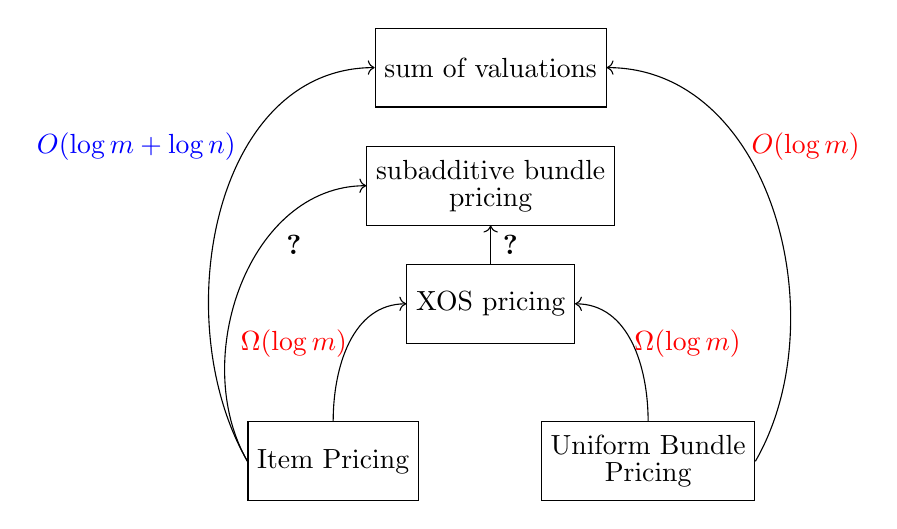
\begin{tikzpicture}
		\node (rectsum) [rectangle, draw, minimum width=7mm, minimum height=10mm] at (0,1.5) {sum of valuations};
		
		\node (rectbundle) [rectangle, draw, minimum width=7mm, minimum height=10mm] at (0,0) {\shortstack{subadditive bundle \\ pricing}};
		
		\node (rectxos) [rectangle, draw, minimum width=7mm, minimum height=10mm] at (0,-1.5) {XOS pricing};
		
		\node (rectitem) [rectangle, draw, minimum width=7mm, minimum height=10mm] at (-2,-3.5) {Item Pricing};
		
		\node (rectubundle) [rectangle, draw, minimum width=7mm, minimum height=10mm] at (2,-3.5) {\shortstack{Uniform Bundle \\ Pricing}};
		
		\draw [->] (rectubundle.east) to [out=60, in = 0] (rectsum);
		\node at (4,0.5) {\textcolor{red}{$O( \log m)$}};
		\draw [->] (rectubundle) to [out=90, in = 0] (rectxos);
		\node at (2.5,-2) {\textcolor{red}{$\Omega( \log m)$}};
		\draw [->] (rectitem.west) to [out=120, in = -180] (rectsum.west);
		\node at (-4.5,0.5) {\textcolor{blue}{$O( \log m + \log n)$}};
		\draw [->] (rectitem) to [out=90, in = -180] (rectxos.west);
		\node at (-2.5,-2) {\textcolor{red}{$\Omega( \log m)$}};
		\draw [->] (rectxos) to  (rectbundle);
		\node at (0.25,-0.75) {\textbf{?}};
		\draw [->] (rectitem.west) [out = 120, in = -180] to  (rectbundle.west);
		\node at (-2.5,-0.75) {\textbf{?}};
		
		\end{tikzpicture}
	}
	\caption{Results Summary: Red font show results in this paper; blue font shows existing known results}
	\label{fig:summary}
\end{figure}

\subsection{Uniform Bundle Pricing}

We begin by proving the $O(\log m)$ upper bound with respect to sum of valuations. 

\begin{lemma}
	Consider a hypergraph $\mH = (\mV, \mE)$ with $m$ edges and valuation $v_e$ for each edge $e \in \mE$. Then, there exists a uniform price $p'$ such that $p^{b}_e = p'$ achieves $O(\log m)$-approximation. 
\end{lemma}
\begin{proof}
	Consider the valuations $v_{e_1}, v_{e_2}, \dots, v_{e_m}$ in increasing order. We claim that $ p^{b}_e  = v_{e_{i'}}$ achieves the desired approximation for some edge $e_{i'}$. Assume for the sake of contradiction that this is not the case. Let $\textsf{OPT} = \sum_{e \in \mE} v_e$. Then $m v_{e_1} < \textsf{OPT}/ \log m$ since we can sell each edge if the bundle price is the smallest valuation. Similarly, $(m - i) v_{e_i} < \textsf{OPT}/ \log m$ for each edge. Adding up all inequalities, we get:
	
	\begin{equation}
	\begin{aligned}
	\textsf{OPT} = \sum_{e \in \mE} v_e & < \frac{\textsf{OPT}}{\log m} (\frac{1}{m} + \frac{1}{m-1} + \dots + 1) \\
	& \leq \textsf{OPT}
	\end{aligned}
	\end{equation}
	
	which is a contradiction.
\end{proof}

Next, we show that the $O(\log m)$ upper bound is tight.

\begin{lemma}
	There exists a set of buyers with XOS valuations such that any uniform bundle price produces revenue atmost $\textsf{OPT}/ \log m$.
\end{lemma}	
\begin{proof}
	Consider $n=m$ items and $m$ buyers such that buyer $b_i$ wants item $i$ for price $1/i$. It is easy to see that the valuations are XOS and achieves a revenue of $\log m$. Consider any fixed $p^b_e = 1/c$ such that $1 \leq c \leq m$. Then, the seller can sell edges that have valuation atleast $1/c$. Observe that the number of such edges is atmost $c$. Therefore, the revenue is atmost $\sum_{e:v_e \leq 1/c} 1/c = O(1)$.
\end{proof}

\subsection{Item Pricing}

Next, we show the $\Omega(\log m)$ gap between item pricing and XOS pricing.

\begin{lemma}
	There exists a set of buyers with XOS valuations such no item pricing solution can obtain revenue better than $\textsf{OPT}/ \log m$.
\end{lemma}
\begin{proof}
	Let $\mC_i$ denote the class of customers that desire exactly $\vert i \vert$ items. We construct the hypergraph instance as follows: Each class of customers $\mC_i$ has exactly $\lceil n/i \rceil$ and each customer in $\mC_i$ is assigned a partition of $i$ items such that no two customers share any item. Thus, the total number of hyperedges is $m = \sum_{i} \vert \mC_i \vert = \Theta( n \log n)$. Figure shows  an instance for $n=6$. We fix the valuation $v_e = 1$ for all hyperedges. This set of valuations is XOS and the revenue obtained by selling each edge at price $p^{b}_e = 1$ extracts the full revenue of $\Theta(n \log n)$.
	
	Next, we show that no item pricing solution can do better than $O(n)$. We will show this by induction on the customer class $\mC_i$. The base case is revenue obtained by selling edges to customers in $\mC_1$. Since there are atmost $n$ edges, the maximum revenue is $O(n)$. Consider the customer class $\mC_k$. Let denote $0 < \alpha \leq 1$ be the fraction of edges sold to customers in $\mC_k$ and let $\mE_k$ denote such edges. Then, the maximum revenue that can be extracted is $\alpha \lceil n/k \rceil$. We distinguish three types of edges: $(i)$ edges that share atleast one item with edges in $\mE_k$ $(ii)$ edges that do not share any item with edges in $\mE_k$ $(iii)$ edges that are strictly contained within $\mE_k$. By the induction hypothesis, the maximum revenue that can be extracted from all type $(ii)$ edges is atmost $O(n)$. Each edge in $\mE_k$ can overlap with atmost $2(k-1)$ edges that have size strictly lesser than $k$. Thus, the revenue extracted from type $(i)$ edges is atmost $2(k-1) \alpha \lceil n/k \rceil = O(n)$. Consider an edge $e' \in \mE_k$ and let $w_1, \dots w_k$ be the weights of items in $e'$. Since the seller is able to sell $e'$, we have that $w_1 + \dots w_k \leq 1$. Observe that the maximum revenue of all edges of size strictly lesser than $k$ (say $k'$) using items in $e'$ is also atmost $w_1 + \dots w_k \leq 1$ which gives revenue of $O(k)$. 
\end{proof}


\section{Experimental Evaluation}

In this section, we will empirically evaluate the performance of known approximation algorithms for item pricing and bundle pricing. Our goal is to understand the behavior of the algorithms on practical \texttt{SQL} queries over real world datasets. We will first describe our experimental setup, followed by the algorithms that we use and various knobs that we can control to create different instances of the hypergraph instances. 

\subsection{Experimental setup}

We perform all our experiments on $2.2$ GHz processor machine with $4$ cores and $16$ GB main memory running OS X $10.10.5$. We use \texttt{MySQL} as our underlying database for query processing and evaluation. Our implementation is written in \textsc{Python} as an enhancement in \textsc{Qirana} prototype system. \textsc{Qirana} generates random neighbors of a database over which query pricing is performed. The advantage of using neighbors is that we can succinctly represent the neighbor without storing the new database, i.e, we can represent the neighbor by storing only the \emph{update query} that generates the neighbor. \textsc{Qirana} generates two types of neighbors: $(i)$ row update; $(ii)$ swap update. A row update changes one attribute of a single tuple and replaces the attribute value with a different value from the specified domain of the particular attribute. For example,  the following row update modifies the \textsf{User.gender} value of the tuple with key $1$ to f to create a neighboring instance of $D$: 

\begin{center}
	\texttt{UPDATE User SET gender = ’f ’ WHERE uid = 1;}
\end{center}

A swap update on the other hand, exchanges the attribute values of $2$ random tuples in a single relation. For example, the following swap update sets
\textsf{User.age} $= 19$ for the tuple with key $1$ and \textsf{User.age} $= 25$ for
the tuple with key $4$:

\begin{center}
\texttt{UPDATE User SET age = 19 WHERE uid = 1;} 

\texttt{UPDATE User SET age = 25 WHERE uid = 4;}
\end{center}

Both row and swap updates generate a neighboring database that is different from $D$. The set of all neighboring databases is called as the \emph{support set} $\mS$. Observe that any \texttt{SQL} query can be expressed as a subset of $\mS$ and vice-versa. More formally,

\begin{proposition}
	Consider the underlying database $D$ and support set $\mS$. Then,
	\begin{enumerate}
		\item Any query $Q$ can be expressed by a unique set $T \subseteq \mS$ such that $T = \{ D' \in \mS \mid Q(D') \neq Q(D)\}$
		\item For any subset $T \subseteq \mS$, there exists a conjunctive query $Q$ such that $T = \{ D' \in \mS \mid Q(D') \neq Q(D)\}$
	\end{enumerate} 
\end{proposition}	

In our framework, given a workload of queries $Q_1, \dots, Q_k$, we define a matrix $M$ of size $k \times |\mS|$ that is initialized as follows, 

\begin{equation}
M[i][j]=\begin{cases}
1, & \text{if $Q_i(D) \neq Q_i(D')$ where $D'$ is the $j^{th}$ neighbor in $\mS$}.\\
0, & \text{otherwise}.
\end{cases}
\end{equation}

Thus, each row in matrix $M$ represents the \emph{disagreement} vector for a query $Q_i$ and can be viewed as a hyperedge where the set of vertices is $\mS$. In other words, matrix $M$ represents a hypergraph $H = (V, E)$ where $V = \mS$ and $E = \{ D' \mid M[i][D'] = 1\}$ for each query $Q_i$ in the workload. Additionally, for each query $Q_i$, we are given a valuation $v_i$ that represents the price a customer is willing to pay for the query. Recall that since our customer is a single minded buyer, we can make the sale only if price $p(Q_i) \leq v_i$. In the following, we will use query and hyperedge interchangeably to simplify the exposition. Without loss of generality, we will also assume that every hyperedge has exactly one customer who wants to purchase it. 

%\subsection{Approximation Algorithms}



\subsection{Experiment Results}

Our first set of experiments is to understand how the approximation algorithms behave on real world queries. The first dataset we use is the $\texttt{\bfseries world}$ dataset, a popular database provided for software developers. It consists of $3$ relations: $\texttt{\bfseries Country}$,$\texttt{\bfseries CountryLanguage}$ and $\texttt{\bfseries City}$ which contain $5000$ tuples and $21$ attributes. We construct a support set of size $15000$ by randomly choosing neighboring databases. The query workload consists of $466$ queries containing selection, projections and join queries with aggregations. We construct the workload by generating changing the predicates in queries. The list of all queries is present in the appendix.

In order to compare different algorithms we use two upper bounds: $(i)$ sum of valuations, and $(ii)$ an upper bound on the optimal subadditive valuation. We find an upper bound on the optimal subadditive valuations by computing a linear program whose constraints encode the bundle arbitrage conditions. Since the number of constraints can be exponential in the number of hyperedges, we optimize by greedily adding constraints for bundles with largest valuations and finding a set of bundles that cover the hyperedge with small valuations. \shaleen{add example}.

\begin{figure*}[t]
	
	\begin{subfigure}{0.45\textwidth} 
		\hspace{-20mm}
		\includegraphics[scale=0.40]{uniformallapproxrealworkload.pdf}
		\caption{Algorithm performance - uniform valuations} \label{fig:uniformapprox}
	\end{subfigure} 
	\begin{subfigure}{0.45\textwidth} 
		\includegraphics[scale=0.40]{histogramhyperedgesize.pdf}
		\caption{Hyperedge size histogram} \label{fig:histogramrealqueries}
	\end{subfigure} 
	\caption{Sampling valuations from uniform distribution}
\end{figure*}
\smallskip
\introparagraph{Sampling from uniform distribution} In our first experiment, we sample valuations from the uniform distribution. Figure~\ref{fig:uniformapprox} shows the performance of all algorithms. The first observation is that uniform bundle pricing outperforms all other algorithms. This is because bundle pricing does not depend on the hyperedge size or structure. For the given query workload, most hyperedges have size between $0$ to $1000$. As we will see later, for bigger sized hyperedges, item pricing performs better.

\begin{figure*}[t]
	
	\begin{subfigure}{0.45\textwidth} 
		\hspace{-20mm}
		\includegraphics[scale=0.40]{zipfianallapproxrealworkload.pdf}
		\caption{Algorithm performance - zipfian distribution} \label{fig:zipfianapprox}
	\end{subfigure} 
	\begin{subfigure}{0.45\textwidth} 
		\includegraphics[scale=0.40]{exponentialallapproxrealworkload.pdf}
		\caption{Algorithm performance - exponential distribution} \label{fig:exponentialapprox}
	\end{subfigure} 
	\caption{Sampling valuations from zipfian and exponential distribution}
\end{figure*}

\smallskip
\introparagraph{Other distributions} Figure~\ref{fig:zipfianapprox} and~\ref{fig:exponentialapprox} perform the same experiment but sample valuation for hyperedges from zipfian and exponential distributions. Uniform bundle pricing is again better than other algorithms and $O(\log B)$-approximation algorithm is marginally better than uniform item pricing LP. Not surprisingly, the layering algorithm does not perform well except in the case of zipfian distribution with exponent smaller than $2$. This is because for $a < 2$, zipfian distribution assigns a large valuation to some hyperedge that contributes significantly to the total revenue. In such cases, the layering algorithm can always extract full revenue from the layer containing high valuation edges and perform well in practice.


% Bibliography
\bibliographystyle{ACM-Reference-Format}
\bibliography{reference}

\end{document}
